\documentclass{report}
\usepackage[T1]{fontenc}
\usepackage[utf8]{inputenc}
\usepackage[francais]{babel}
\usepackage{amsmath}
\usepackage{graphicx}
\usepackage[backend=biber,style=authoryear,bibencoding=utf8]{biblatex}
\usepackage[colorlinks,linkcolor=blue]{hyperref}

\addbibresource{biblio.bib}

\begin{document}
\chapter*{MRTF-A}
En 2001, \cite{mercher_involvement_2001} 
décrivent une translocation impliquée dans les leucémies aigües mégacaryocytiques. 
Il s'agit de la translocation d'un gène du chromosome 1 sur le chromosome 22, le gène fusion est nommmé One-Twenty-Two-Megakaryocytic-Acute-Leukemia (OTT-MAL). 
Les fonctions des deux gènes qui ont fusionné est alors inconnue. 

En 2002, deux homologues de la myocardine sont identifiés dans le génome humain par \cite{wang_potentiation_2002} et sont nommés Myocardin-Related Transcription Factor A et B (MRTF-A/B).
MRTF-A correspond au gène du chromosome 22 MAL (ou MKL1) et MRTF-B à un gène du chromosome 16 (MAL16 ou MKL2). 
Un homologue est également découvert chez la souris et nommé Basic, SAP et Coil-coil (BSAC) \parencite{sasazuki_identification_2002}. 

Alors que cette protéine sera appelée dans la suite de ce document MRTF-A, elle pourra être identifiée indifféremment comme MAL, MKL1 ou BSAC dans la bibliographie. 

\section{MRTF-A, cofacteur de Serum Response Factor}

La fonction principale des protéines de la famille des myocardines est l'activation du facteur de transcription Serum Response Factor. 

\subsection{Serum Response Factor}

Serum Response Factor est un facteur de transcription qui fait partie de la famille MADS (MCM-1, Agamous, Deficiens, SRF). SRF est présent en un seul exemplaire dans le génome humain mais peut être transcrit en 4 isoformes. 
La protéine SRF comprend un signal de localisation nucléaire (NLS), une boîte MADS composée du site de liaison à l'ADN et d'un domaine de dimérisation, et d'un domain de transactivation auquel se fixent ses cofacteurs. 

Un dimère SRF se fixe sur une séquence consensus de nucléotides sur l'ADN appelée boîte CArG : CC(A/T)$_{6}$GG, ou sur une séquence CArG-like, qui diffère du consensus d'une seule base, avec une affinité plus faible. Le gène srf contenant lui-même deux boîtes CArG, il est sa propre cible, dans une boucle de rétro-action positive. 

\subsection{Les cofacteurs de SRF : TCF et MRTF}

Serum Response Factor n'est lui-même qu'un transactivateur faible, mais il peut être activé par deux grandes familles de cofacteurs : les Ternary Complex Factors, et les Myocardin-Related Transcription Factor. 

Les deux familles ne sont pas concurrentes pour se lier à SRF : la plupart des sites sur l'ADN sont spécifiques de l'une ou l'autre des familles de cofacteurs (\cite{esnault_rho-actin_2014}). Même lorsque les MRTF sont séquestrées dans le cytoplasmes, les TCF ne les remplacent pas sur les sites de liaison à SRF. 

Un ChIP-seq sur des fibroblastes 3T3 a estimé que 921 gènes sont susceptibles d'être régulés par MRTF/SRF en réponse au sérum, et 76 gènes par TCF/SRF (\cite{esnault_rho-actin_2014}), ce qui représente entre 3 et 4\% du génome. Les MRTF sont donc un élément important de la régulation transcriptionnelle, et l'acteur principal de la régulation de SRF. 

\emph{Les autres cofacteurs de SRF ? }

\section{MRTF-A, indépendamment de SRF}

\subsection{Transition épithélio-mésenchymateuse et domaine SAP}
\subsection{NF-$\kappa$B}


\subsubsection{Ternary Complex Factors}

Elk1, Net et SAP-1 sont trois coactivateurs de SRF de la même famille, les TCF. Ils possèdent un domaine qui leur permet de se lier à des sites spécifiques sur l'ADN (Ets Binding Sites). 
Lorsqu'un site Ets et une boîte CArG sont adjacents, ils forment un Serum Response Element (SRE). La formation d'un complexe TCF-SRF sur un SRE déclenche la transcription du gène cible. 

Les TCF sont phosphorylées et activées par les MAPK (Mitogen Activated Protein Kinases). 


\subsubsection{La famille Myocardine}

Cette famille de cofacteurs de SRF comprend la myocardine, MRTF-A et MRTF-B. 

La myocardine se présente sous deux isoformes, une forme cardiaque et une forme spécifique au muscle lisse. Les deux sont exclusivement localisées dans le noyau et sont constitutivement actives, en raison de motifs RPEL déficients ou incomplets. 

Les Myocardin-Related Transcription Factors A et B sont exprimées dans un grand nombre de tissus : muscles cardiaques, lisses et squelettiques, neurones, cellules épithéliales, mégacaryocytes \dots Contrairement à la myocardine, les MRTF peuvent être séquestrées dans le cytoplasme, ce qui les empêche d'activer SRF et la transcription. La régulation de la localisation de MRTF est assurée par l'actine, qui peut former un complexe avec la partie N-terminale des MRTF. 

One-Twenty-Two-Megakaryocytic-Acute-Leukemia (OTT-MAL) est la protéine résultant d'une translocation d'un gène du chromosome 1 à côté du gène MRTF-A. La protéine fusion comprend presque toute la protéine MRTF-A excepté la partie N-terminale. 


\section*{Structure de MRTF-A}

\begin{figure}
\center
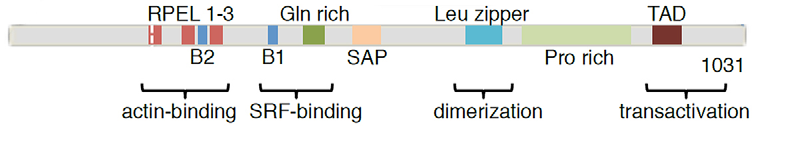
\includegraphics[scale=0.5]{MRTFA_structure.png}
\caption{Structure de MRTF-A \parencite{scharenberg_tgf-_2014}}
\end{figure}
 \subsection{Les motifs RPEL}
 
 La partie N-terminale de MRTF-A contient trois motifs RPEL consécutifs, qui peuvent se lier aux monomères d'actine (\cite{posern_mutant_2004}, \cite{mouilleron_molecular_2008}) avec des affinités variables, les deux premiers motifs se liant plus fortement que le troisième (\cite{guettler_rpel_2008}). La structure détaillée du complexe montre que les trois motifs RPEL se lient à 3 à 5 monomères d'actine selon la concentration en monomères d'actine. (\cite{hirano_sensing_2011}, \cite{treisman_structure_2011}). 
 
 Deux domaines basiques, B2 et B3 sont inclus dans les motifs RPEL et forment un signal de localisation nucléaire (NLS) bipartite (\cite{rajakyla_actin-regulated_2010}). Lorsqu'il n'y a pas d'actine sur les motifs RPEL, ce NLS peut se lier au complexe Importine$\alpha / \beta$ (\cite{hirano_sensing_2011},\cite{rajakyla_actin-regulated_2010}) et MRTF-A est importée dans le noyau de la cellule, où se trouve SRF. En présence de suffisamment de monomères, le NLS est recouvert par l'actine liée aux RPEL, MRTF-A reste cytoplasmique (Posern 2002, \cite{miralles_actin_2003},\cite{posern_mutant_2004}). 
 
 MRTF-A est exportée du noyau par Crm1 (\cite{vartiainen_nuclear_2007},\cite{hayashi_differences_2013}). \emph{Ces deux articles se contredisent sur la question de la liaison à l'actine : le premier prétend qu'elle est indispensable, le second qu'elle empêche l'export} 
 
 Les motifs RPEL sont donc la clé de la régulation de MRTF-A par l'actine : selon la concentration en monomères d'actine, MRTF-A est localisée dans le cytoplasme en cas d'excès et dans le noyau, où se trouve SRF, en cas de manque. Lorsque le domaine RPEL est muté ou absent, la protéine est constitutivement nucléaire (\cite{miralles_actin_2003}), comme la myocardine, dont les motifs RPEL ne sont plus fonctionnels (\cite{guettler_rpel_2008}). 
 
 \subsection{La région basique et SRF}
 La région B1 est le site de liaison de MRTF-A à SRF. MRTF-A s'attache préférentiellement à SRF en dimère (\cite{miralles_actin_2003}). Le complexe MRTF-A-5actines ne peut pas se lier à SRF et l'activer, la présence de MRTF-A dans le noyau n'est donc pas suffisante pour activer SRF, il faut également que la concentration en G-actine dissocie le complexe (\cite{vartiainen_nuclear_2007}). 
 \subsection{Leucine zipper et oligomérisation}
 MRTF-A/B peuvent former des homo ou des hétérodimères (\cite{miralles_actin_2003}). Un dominant négatif pourra ainsi bloquer une protéine WT dans un hétérodimère non fonctionnel (\cite{selvaraj_megakaryoblastic_2003},\cite{cen_myocardin/mkl_2004}, \cite{li_requirement_2005},\cite{rajakyla_actin-regulated_2010}). La formation des dimères n'est pas indispensable à la fonctionnalité de MRTF-A, les mutations dans cette région réduisent son efficacité sans l'inhiber totalement (\cite{selvaraj_megakaryoblastic_2003}). 
 OTT-MAL est également capable de former des hétérodimères avec les MRTF, et donc de perturber leur équilibre. 
 
 \subsection{SAP et TAD}
 
Dans les cellules épithéliales, il a été montré qu'un groupe de gènes est activé par MRTF-A et nécessite particulièrement la zone SAP, tout en étant indépendant de SRF (\cite{asparuhova_transcriptional_2011}, \cite{gurbuz_sap_2014}) 
 
 \subsection{Phosphorylation}
	MRTF-A peut être phosphorylée (\cite{miralles_actin_2003},\cite{cen_myocardin/mkl_2004},).Dans les neurones, la phosphorylation de MRTF-A par ERK1/2 est même la voie principale de régulation de son activité, car la protéine est toujours nucléaire, mais elle n'active SRF qu'une fois phosphorylée (\cite{kalita_role_2006}).
	
 \subsection{Isoformes}
 D'après \cite{scharenberg_tgf-_2014}, il existe 2 isoformes de MRTF-A chez l'humain, une version longue (MRTF-A\_L) et une courte(MRTF-A\_S). La version longue présente 80 acides aminés avant le premier motif RPEL, contre 15 seulement pour la version courte. Cette dernière contient deux TAD de 9 acides aminés (9aaTAD), un à l'extrémité C-terminale, et un à l'extrémité N-terminale spécifique à cet isoforme. Une surexpression de MRTF-A\_S est observée en réponse à TGF-$\beta$ ou à une contrainte cyclique dans les cellules épithéliales. 
 
 

\section{Rôles de MRTF-A}
Depuis sa découverte au début des années 2000, de nombreux rôles de MRTF-A ont été mis en évidence dans des types cellulaires et dans des tissus très divers. 
\subsection{Embryogenèse}

Les MRTF sont exprimées dès le jour 10 du développement de l'embryon (\cite{wang_potentiation_2002}), dans tous les tissus. La délétion de MRTF-B entraîne l'échec de la gastrulation, et donc une fin précoce de l'embryogenèse (\cite{kalita_mkls:_2012}). Au contraire, 60\% des mutants MRTF-A$^{-/-}$ sont viables et atteignent l'âge adulte, les autres étant perdus pendant l'embryogenèse car souffrant de défauts cardiaques. Les mutants survivants sont dépourvus de ces anomalies cardiaques, et vivent jusqu'à l'âge adulte (\cite{li_requirement_2006},\cite{sun_acute_2006}). Cependant, les femelles souffrent d'un défaut de formation de la glande mammaire,  lié à une apoptose précoce des cellules myoépithéliales qui déclenchent l'éjection du lait. Il apparaît donc que chez la souris, tandis que MRTF-B est indispensable à l'embryogenèse, l'absence de MRTF-A peut être compensée dans la plus grande partie des tissus. 
Les souris possédant un gène mutant dominant négatif de MRTF-A sont en revanche de plus petite taille, ne bougent pas et ne survivent que quelques jours, principalement à cause des défauts de musculature de leur diaphragme (\cite{li_requirement_2005}). 

\subsection{Régulation de la masse musculaire}

Serum Response Factor a pour gènes cibles un grand nombre de gènes liés au cytosquelette et à la différenciation musculaire. 

Lorsque SRF est désactivé dans le muscle squelettique de souris adulte ( souris HSA-Cre-ER$^T2$:srf$^{flox/flox}$ ), l'hypertrophie compensatoire de ses muscles est bloquée (\cite{guerci_srf-dependent_2012}). Les cellules satellites sont moins nombreuses, et ne fusionnent pas avec les fibres musculaires. Au contraire, un SRF constitutivement actif protège de l'atrophie liée à une immobilisation ou à une dénervation. 
Suite à une dénervation, MRTF-A est exclus des noyaux des fibres musculaires, et donc incapable d'activer SRF. Un MRTF-A constitutivement nucléaire protège contre l'atrophie induite par la dénervation(\cite{collard_nuclear_2014}). C'est donc la régulation de la localisation de MRTF-A dans les fibres musculaires qui régule l'activité de SRF et l'atrophie ou l'hypertrophie en réponse aux contraintes mécaniques.  


Dans les myoblastes murins C2C12, un domninant négatif MRTF-B, capable d'interférer avec l'activité des deux MRTF, bloque la différenciation musculaire en myotubes et diminue leur taux de duplication (\cite{selvaraj_megakaryoblastic_2003}, \cite{cen_megakaryoblastic_2003}). 
Les souris DN-MRTF-A montrent d'ailleurs un phénotype myopathique. 




\subsection{Transition épithéliale-mésenchymale}

La transition épithélio-mésenchymateuse est le processus par lequel des cellules, sous l'influence de signaux extérieurs, vont perdre leur type épithélial (expression de l'E-cadherine, polarisation, organisation en monocouche jointive \dots) et acquérir un phénotype mésenchytmal (expression de N-cadherine, motilité plus importante, fabrication de matrice extra-cellulaire \dots). 
Plusieurs marqueurs de l'EMT, comme la vimentine ou l'actine du muscle lisse $\alpha$Smooth Muscle Actin sont des cibles de SRF. 

La conjonction d'un signal biochimique, TGF $\beta$ (Transforming Growth Factor), et d'un signal mécanique déclenche l'activation de la voie de signalisation RhoA/actine/MRTF-A/SRF. 
Les signaux mécaniques déclencheurs peuvent être très divers, locaux ou globaux, cycliques ou statiques : membranes étirées cycliquement (\cite{maier_tenascin-c_2008}), ilôts de fibronectine  (\cite{gomez_tissue_2010},\cite{connelly_actin_2010}), gels de polyacrylamides de différentes rigidités (\cite{huang_matrix_2012}), microbilles magnétiques recouvertes de collagène (\cite{chan_force-induced_2010}). 



\subsection{MRTF-A et cancers}




\newpage


\section{En amont de MRTF-A : voie de signalisation et régulation de l'actine} 
\subsection{Régulation de l'actine}
\subsection{Les protéines liées à l'actine}
\subsection{La voie RhoA}
\subsection{MICAL2}

\section{En aval de MRTF-A : SRF et gènes cibles}

%\printbibliography
\end{document}